\chapter{Smith-Whitten Coordinates}\label{smith}
\section{Coordinate Mapping}\label{Appendix_2_1}
Johnson has given a detailed description of how the three-body system can be represented in a symmetric way \cite{Johnson1980}. In this section we present the main procedures used to retrieve a mapping for the three-dimensional triatomic potential energy surface to a point in configuration space. This mapping will treat the different arrangement channels equally, which enables permutation symmetries for three identical particles to be imposed exactly. Performing a second mapping of the original representation presented in \cite{Smith1962,Smith_Whitten1968} yields the resulting set of modified Smith-Whitten coordinates. The derivation of the Hamiltonian for this representation is then described in \cref{Appendix_2_2}. Some of the definitions presented in \cref{MNJC} will be repeated here in oredr for this appendix to be complete.

Let $\mathbf{x}_i$ and $m_{i}$ be the position vector and mass of the $i$th particle in the laboratory frame. If the total mass $M$, the three particle reduced mass $\mu$, and the normalizing constants $d_{k}$ $(k=1,2,3)$ are given by

\begin{align}
M &= \sum_{i=1}^{3}m_i, \\
\mu^2 &= \prod_{i=1}^{3}m_i/M,\\
d_k^2 &= \frac{m_k}{\mu}\frac{(m_i+m_j)}{M},
\end{align}
then the set of mass-scaled Jacobi vectors and the center of mass coordinate can be defined as

\begin{align}
\mathbf{r}_k &= d^{-1}_k(\mathbf{x}_{j}-\mathbf{x}_{i}), \\
\mathbf{R}_k &= d_k\Big[\mathbf{x}_{k}-\frac{(m_{i}\mathbf{x}_{i}+m_{j}\mathbf{x}_{j})}{m_{i}+m_{j}}\Big],\\
\mathbf{X}_{CM} &= \frac{1}{M} \sum_{i=1}^{3} m_{i} \mathbf{x}_{i},
\end{align}   
in which, the indices $i,j,k$ are cyclic permutations of $(1,2,3)$. The center-of-mass is separated out and will not be considered further. Transformations within the set of coordinates is aided by defining the angle $\beta_{ij}$, which have the following properties

\begin{subequations}
	\begin{align}
	&\beta_{ij} = -\beta_{ji}, \quad \beta_{ii} = 0,\\
	&\tan\beta_{ij} = -m_k/\mu,\\
	&d_{i}d_{j} \sin\beta_{ij} = 1,\\
	&d_{i}d_{j} m_{k} \cos\beta_{ij} = -\mu,\\
	&\beta_{12}+\beta_{23}+\beta_{31} = 2\pi.
	\end{align}
\end{subequations}
Orthogonal transformations are then given by 

\begin{equation}\label{eq:kinematic_rot}
\begin{pmatrix}
\mathbf{r}_j\\
\mathbf{R}_j
\end{pmatrix}
=
\begin{pmatrix}
\cos\beta_{ij} & \sin\beta_{ij}\\
-\sin\beta_{ij} & \cos\beta_{ij}
\end{pmatrix}
\begin{pmatrix}
\mathbf{r}_i\\
\mathbf{R}_i
\end{pmatrix}.
\end{equation}   

To define a symmetric coordinate system, one starts by separating the external and internal coordinates of the configuration. For the external coordinates we use the Euler angles, these are used to relate rotations of the three-body system in space. Since the potential energy only depends on the internal coordinates we will focus on them here. The internal coordinates $\rho$, $\Theta$, and $\Phi_k$ determine the size, shape and particle arrangement of the triangle formed by the three-body system, respectively. Starting from the definition for the internal coordinates given by Smith and Whitten \cite{Smith_Whitten1968}

\begin{equation}
	\begin{aligned}
	r_x^k &= \rho \cos\Theta\cos\Phi_k,\\
	r_y^k &= -\rho \sin\Theta\sin\Phi_k,\\
	r_z^k &= 0\\
	R_x^k &= \rho \cos\Theta\sin\Phi_k,\\
	R_y^k &= \rho \sin\Theta\cos\Phi_k,\\
	R_z^k &= 0,
	\end{aligned}   
\end{equation}
where $\Phi_k$ is in the range $0 \leq \Phi_k < 2\pi$ and $\Theta$ is in the range $0 \leq \Theta \leq \pi/4$. The distances between the particles $ij$ are related through 

\begin{equation}
r_{ij} = \abs{\mathbf{x}_j - \mathbf{x}_i} = d_k \abs{\mathbf{r}_k} = \frac{d_k\rho}{2^{1/2}}\big[1 + \cos(2\Theta)\cos(2\Phi_k)\big]^{1/2}.
\end{equation}
The kinematic rotations \eqref{eq:kinematic_rot} correspond to the following transformation in hyperspherical space 

\begin{equation}
	\Phi_j = \Phi_i-\beta_{ij}.
\end{equation}
This is easily shown by performing transformations within the coordinate set. If we choose $k=3$ then 

\begin{equation}
\begin{aligned}
r_{12} = d_3 \mid\mathbf{r}_{3}\mid &= \frac{\rho d_3}{2^{1/2}}\big[1+\cos(2\Theta)\cos(2\Phi_3)\big]^{1/2}\\
r_{23} = d_1 \mid\mathbf{r}_{1}\mid &= d_1 \big[\cos^2\beta_{31}\mathbf{r}^2_{3} + \sin^2\beta_{31}\mathbf{R}^2_3 + 2\sin\beta_{31}\cos\beta_{31}\mathbf{r}_3\cdot\mathbf{R}_3\big]^{1/2}\\
&= \frac{d_1\rho}{2^{1/2}} \big[\cos^2\beta_{31}(1 + \cos(2\Theta)\cos(2\Phi_3))\\ 
&+ \sin^2\beta_{31}(1 - \cos(2\Theta)\cos(2\Phi_3))\\ 
&+ 2\sin\beta_{31}\cos\beta_{31}\cos(2\Theta)\sin(2\Phi_3)\big]^{1/2}\\ 
&= \frac{d_1\rho}{2^{1/2}} \big[1 + \cos(2\Theta)\big(\cos(\Phi_3)\cos(2\beta_{31}) + \sin(2\Phi_3)\sin(2\beta_{31})\big)\big]^{1/2}\\ 
&= \frac{d_1\rho}{2^{1/2}}\big[1 + \cos(2\Theta)\cos(2\Phi_3 - 2\beta_{31})\big]^{1/2}\\ 
&= \frac{d_1\rho}{2^{1/2}}\big[1 + \cos(2\Theta)\cos(2\Phi_1)\big]^{1/2}\\ 
r_{31} = d_2 \mid\mathbf{r}_{2}\mid
&= d_2 \big[\cos^2\beta_{23}\mathbf{r}^2_{3} + \sin^2\beta_{23}\mathbf{R}^2_3 - 2\sin\beta_{23}\cos\beta_{23}\mathbf{r}_3\cdot\mathbf{R}_3\big]^{1/2}\\ 
&= \frac{d_2\rho}{2^{1/2}} \big[1 + \cos(2\Theta)\big(\cos(\Phi_3)\cos(2\beta_{23}) - \sin(2\Phi_3)\sin(2\beta_{23})\big)\big]^{1/2}\\ 
&= \frac{d_2\rho}{2^{1/2}}\big[1 + \cos(2\Theta)\cos(2\Phi_3 + 2\beta_{23})\big]^{1/2}\\
&= \frac{d_2\rho}{2^{1/2}}\big[1 + \cos(2\Theta)\cos(2\Phi_2)\big]^{1/2}.
\end{aligned}
\end{equation}
By defining

\begin{equation}
\begin{aligned}
\epsilon_1 &= -2\tan^{-1}(-m_2/\mu)\\
\epsilon_2 &= 2\tan^{-1}(-m_1/\mu).
\end{aligned}
\end{equation} 
These the distances are given by 

\begin{equation}
\begin{aligned}
r_{12} &= \frac{d_3\rho}{2^{1/2}}\big[1+\cos(2\Theta)\cos(2\Phi)\big]^{1/2}\\
r_{23} &= \frac{d_1\rho}{2^{1/2}}\big[1 + \cos(2\Theta)\cos(2\Phi + \epsilon_1)\big]^{1/2}\\
r_{31} &= \frac{d_2\rho}{2^{1/2}}\big[1 + \cos(2\Theta)\cos(2\Phi + \epsilon_2)\big]^{1/2}
\end{aligned}
\end{equation}
where the angular indice $3$ is surpressed.

Kuppermann pointed out that there are some disadvantages with this representation \cite{KUPPERMANN1975374}. For the mapping of the triatomic potential energy surface to configuration space, we require that every internal configuration corresponds to one point only and that a transformation of $\Phi_k$ and $\Theta$ should rotate, but not distort, the equipotential surface about the $z$-axis. Because each particle arrangement corresponds to two points in the hyperspherical coordinate space within the range of the hyperangles, we perform a second mapping

\begin{equation}
\begin{aligned}
\theta &= \pi/2-2\Theta,\\
\tilde{\phi}_k &= \pi/2-2\Phi_k,
\end{aligned}
\end{equation}
where the ranges of these new coordinates are 

\begin{equation}
\begin{aligned}
0  &\leq \theta \leq \pi/2,\\
-7\pi/2 &\leq \tilde{\phi}_k < \pi/2,
\end{aligned}
\end{equation} 
and the distances are subsequently given by

\begin{equation}
r_{ij} = \frac{d_k\rho}{2^{1/2}}\big[1 + \sin\theta\sin\tilde{\phi}_k\big]^{1/2}.
\end{equation}
To get a more conveinient range we redefine $\phi_k = \tilde{\phi}_k+7\pi/2$, so that the range is $0 \leq \phi_k < 4\pi$. Then we finally get

\begin{equation}
r_{ij} = \frac{d_k\rho}{2^{1/2}}\big[1 + \sin\theta\cos\phi_k\big]^{1/2},
\end{equation}
where the corresponding kinetic rotations are $\phi_j=\phi_i-2\eta_{ij}$, in which the angle $\eta_{ij}$ $(2\eta_{ij} = -2\beta_{ij})$ is in the range $0 \leq \eta_{ij} \leq \pi/2$ and have the properties

\begin{subequations}
\begin{align}
&\eta_{ij} = -\eta_{ji}, \quad \eta_{ii} = 0,\\
&\tan\eta_{ij} = m_k/\mu,\\
&\eta_{12}+\eta_{23}+\eta_{31} = \pi.
\end{align} 
\end{subequations}

If the cartesian coordinates of this point in configuration space is defined to be the regular spherical polar coordinates, then all configurations will map to the upper half-space $z \geq 0$ (since $z_k=\rho\cos\theta$ and $0\leq \theta \leq \pi/2$). Since $\phi_k$ and $\phi_k + 2\pi$ represent the same internal configuration and also points to the same point in configuration space, each point in the upper half-space represent a unique arrangement of the three-body system. Exchanging two of the particles will generate a new arrangement, which coorseponds to a new point in configuration space. 

We can choose one of the branches of $\phi_k$ by restricting the range to $0 \leq \phi_k < 2\pi$. Finally, we choose the Jacobi coordinates where $k=3$ and subsequently get the expression for our hyperspherical coordinates

\begin{equation}
\begin{aligned}
r_{12} &= \frac{d_3\rho}{2^{1/2}}\big[1+\sin\theta\cos\phi\big]^{1/2}\\
r_{23} &= \frac{d_1\rho}{2^{1/2}}\big[1 + \sin\theta\cos(\phi-\varphi_1)\big]^{1/2}\\
r_{31} &= \frac{d_2\rho}{2^{1/2}}\big[1 + \sin\theta\cos(\phi + \varphi_2)\big]^{1/2},
\end{aligned}
\end{equation}
in which

\begin{equation}
\begin{aligned}
\varphi_1 &= 2\tan^{-1}(m_2/\mu),\\
\varphi_2 &= 2\tan^{-1}(m_1/\mu).
\end{aligned}
\end{equation}

In \cref{fig:potential} the triatomic potential energy surface for the model potential used in \cref{smith_whitten}, see \cref{eq:two_b_potential,eq:potential_sum}, is shown for three identical particles. As seen in the figure, the translation and reflection symmetries reduce the range of $\phi$ once more to $0 \leq \phi < \pi/3$ for identical particles. 

\begin{figure}
	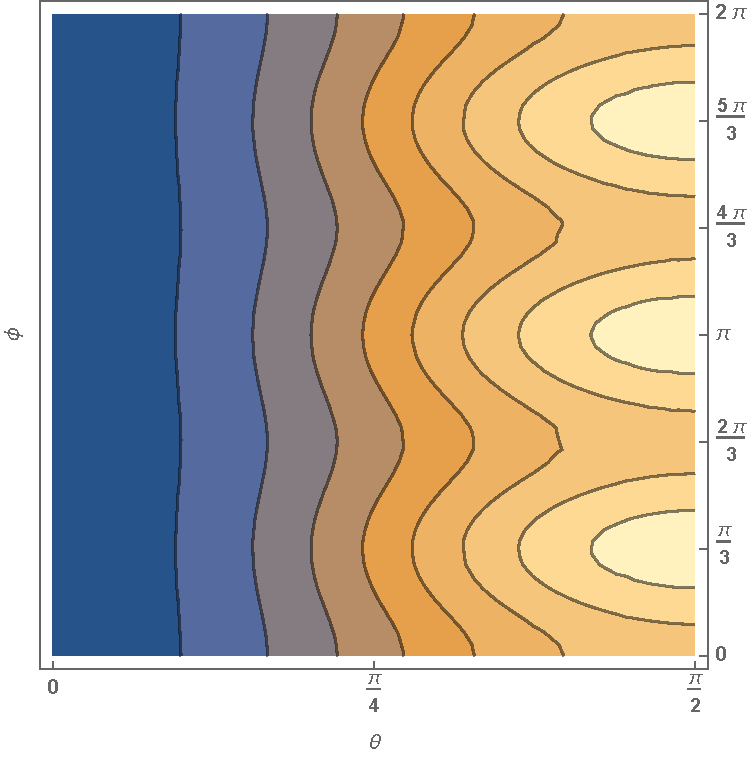
\includegraphics[width=\linewidth]{potential.pdf}
	\caption{Potential surface for three identical particles. Symmetries due to translations and reflections are seen at $\phi = n\pi/3, \ (n = 1-5)$.}
	\label{fig:potential}
\end{figure}
